\section{Time Transactions}
\label{section:time_transactions}

\begin{figure}[H]
\centering
\includegraphics[scale=0.60]{05_time_transactions/png/time_transaction}
\caption{Time Transactions}
\label{fig:time_transactions2}
\end{figure}

\subsection{Including Time Transactions in Our Model}

\begin{figure}[H]
\centering
\includegraphics[scale=0.60]{05_time_transactions/png/time_transaction_feedback_schema}
\caption{Exchange and Time Transaction Feedback Schema}
\label{fig:exchange_and_time_transaction_schema1}
\end{figure}

\subsection{Interaction of Time Transactions and Exchange Transactions}

\underline{Introduction}

\underline{Units}




\underline{Inflation Feedback}

Increases in the inflation rate driven through exchange transactions has effects on time
transactions. We demonstrate in section (\ref{section:exchange_transactions_and_errors}) we showed
that an error rate limits the equilibriation process. We now show an interaction between time
transactions and exchange transactions that has further effects the equilibriation process by
driving down growth rates.

This process generates a positive and unstable feedback loop between exchange transactions and time
transactions. We will show how increases in the inflation rate cause increases in real interest
rates, and by pushing up the costs of production, reduce the growth rates. As show in section
(\ref{section:exchange_transactions_and_errors}) this will either increase the inflation rate,
increasing the effect of the positive feedback process, or increase the unemployment rate. The
positive feedback loop is broken only when increases in the inflation rate cease.  

\underline{The feedback process}

In Chapter V (pages 77-   ) of his 1907 work \textit{The Rate of Interest} Irving Fisher examines an
adjustment that economic participants must make to nominal interest rates if they are to maintain
real interest rates at a certain fixed rate, under inflationary conditions.

If we have a time-transaction that occurs at a time when the borrower and lender expect not change
in the price-level, and the borrowser and lender agree on a real interest rate of $i$ percent, then
a repayment of the priniciple $k$ will be repaid together with an interest payment of $ki$, making a
total repayment of $k(1+i)$.

If the lender and borrow want to carry out the same transaction in times when the borrower and
lender expected the price level to increase by $I$ percent by the time the repayment was due, then
the borrower and lender could carry out the same transaction, by repaying principle at $k(1+I)$ with
an interest payment of $ki(1+I)$, making a total repayment of $k(1+i)(1+I)$.

Regardless of which or these two circumstances is the case, the payments are the same if we adjust
for changes in the price level.

 





If $k$ units of currency is lent at a time time when the inflation rate

If $k$ units of currency are lent at a time where the price level is $p_0$ and buyers expect that at
the time of repayment the price level will have rise $I$ percent, then







This is a process which in addition together with the effect of an error rate on market equilibrium
accounts for most of the effects of currency on market stability equilibrium and stability.


